\documentclass[10pt]{article}


\usepackage{times}
\usepackage{amsfonts}
\usepackage{amsmath}
\usepackage[psamsfonts]{amssymb}
\usepackage{latexsym}
\usepackage{color}
\usepackage{graphics}
\usepackage{enumerate}
\usepackage{amstext}
\usepackage{blkarray}
\usepackage{url}
\usepackage{epsfig}
\usepackage{bm}
\usepackage{hyperref}
\hypersetup{
    colorlinks=true,
    linkcolor=blue,
    filecolor=magenta,      
    urlcolor=blue,
}
\usepackage{mathtools}
 

%% Probability operators and functions
%
% \def \P{\mathrm{P}}
\def \P{\mathrm{P}}
\def \E{\mathrm{E}}
\def \Var{\mathrm{Var}}
\let\var\Var
\def \Cov {\mathrm{Cov}} \let\cov\Cov
\def \MSE {\mathrm{MSE}} \let\mse\MSE
\def \sgn {\mathrm{sgn}}
\def \R {\mathbb{R}}
\def \C {\mathbb{C}}
\def \N {\mathbb{N}}
\def \Z {\mathbb{Z}}
\def \cV {\mathcal{V}}
\def \cS {\mathcal{S}}
\DeclareMathOperator*{\argmin}{arg\,min}
\DeclareMathOperator*{\argmax}{arg\,max}
\newcommand{\red}[1]{\textcolor{red}{#1}}
\newcommand{\blue}[1]{\textcolor{blue}{#1}}
\newcommand{\green}[1]{\textcolor{ForestGreen}{ #1}}
\newcommand{\fuchsia}[1]{\textcolor{RoyalPurple}{ #1}}

%
%% Probability distributions
%
%\def \Bern    {\mathrm{Bern}}
%\def \Binom   {\mathrm{Binom}}
%\def \Exp     {\mathrm{Exp}}
%\def \Geom    {\mathrm{Geom}}
%\def \Norm    {\mathcal{N}}
%\def \Poisson {\mathrm{Poisson}}
%\def \Unif    {\mathrm {U}}
%
\newcommand{\bdb}[1]{\textcolor{red}{#1}}

\newcommand{\ml}[1]{\mathcal{ #1 } }
\newcommand{\wh}[1]{\widehat{ #1 } }
\newcommand{\wt}[1]{\widetilde{ #1 } }
\newcommand{\conj}[1]{\overline{ #1 } }
\newcommand{\rnd}[1]{\tilde{ #1 } }
\newcommand{\rv}[1]{ \rnd{ #1}  }
\newcommand{\rx}{\rnd{ x}  }
\newcommand{\ry}{\rnd{ y}  }
\newcommand{\ra}{\rnd{ a}  }
\newcommand{\rb}{\rnd{ b}  }
\newcommand{\rpc}{\widetilde{ pc}  }

\def \cnd {\, | \,}
\def \Id { I }
\def \J {\mathbf{1}\mathbf{1}^T}

\newcommand{\op}[1]{\operatorname{#1}}
\newcommand{\setdef}[2]{ := \keys{ #1 \; | \; #2 } }
\newcommand{\set}[2]{ \keys{ #1 \; | \; #2 } }
\newcommand{\sign}[1]{\op{sign}\left( #1 \right) }
\newcommand{\trace}[1]{\op{tr}\left( #1 \right) }
\newcommand{\tr}[1]{\op{tr}\left( #1 \right) }
\newcommand{\inv}[1]{\left( #1 \right)^{-1} }
\newcommand{\abs}[1]{\left| #1 \right|}
\newcommand{\sabs}[1]{| #1 |}
\newcommand{\keys}[1]{\left\{ #1 \right\}}
\newcommand{\sqbr}[1]{\left[ #1 \right]}
\newcommand{\sbrac}[1]{ ( #1 ) }
\newcommand{\brac}[1]{\left( #1 \right) }
\newcommand{\bbrac}[1]{\big( #1 \big) }
\newcommand{\Bbrac}[1]{\Big( #1 \Big)}
\newcommand{\BBbrac}[1]{\BIG( #1 \Big)}
\newcommand{\MAT}[1]{\begin{bmatrix} #1 \end{bmatrix}}
\newcommand{\sMAT}[1]{\left(\begin{smallmatrix} #1 \end{smallmatrix}\right)}
\newcommand{\sMATn}[1]{\begin{smallmatrix} #1 \end{smallmatrix}}
\newcommand{\PROD}[2]{\left \langle #1, #2\right \rangle}
\newcommand{\PRODs}[2]{\langle #1, #2 \rangle}
\newcommand{\der}[2]{\frac{\text{d}#2}{\text{d}#1}}
\newcommand{\pder}[2]{\frac{\partial#2}{\partial#1}}
\newcommand{\derTwo}[2]{\frac{\text{d}^2#2}{\text{d}#1^2}}
\newcommand{\ceil}[1]{\lceil #1 \rceil}
\newcommand{\Imag}[1]{\op{Im}\brac{ #1 }}
\newcommand{\Real}[1]{\op{Re}\brac{ #1 }}
\newcommand{\norm}[1]{\left|\left| #1 \right|\right| }
\newcommand{\norms}[1]{ \| #1 \|  }
\newcommand{\normProd}[1]{\left|\left| #1 \right|\right| _{\PROD{\cdot}{\cdot}} }
\newcommand{\normTwo}[1]{\left|\left| #1 \right|\right| _{2} }
\newcommand{\normTwos}[1]{ \| #1  \| _{2} }
\newcommand{\normZero}[1]{\left|\left| #1 \right|\right| _{0} }
\newcommand{\normTV}[1]{\left|\left| #1 \right|\right|  _{ \op{TV}  } }% _{\op{c} \ell_1} }
\newcommand{\normOne}[1]{\left|\left| #1 \right|\right| _{1} }
\newcommand{\normOnes}[1]{\| #1 \| _{1} }
\newcommand{\normOneTwo}[1]{\left|\left| #1 \right|\right| _{1,2} }
\newcommand{\normF}[1]{\left|\left| #1 \right|\right| _{\op{F}} }
\newcommand{\normLTwo}[1]{\left|\left| #1 \right|\right| _{\ml{L}_2} }
\newcommand{\normNuc}[1]{\left|\left| #1 \right|\right| _{\ast} }
\newcommand{\normOp}[1]{\left|\left| #1 \right|\right|  }
\newcommand{\normInf}[1]{\left|\left| #1 \right|\right| _{\infty}  }
\newcommand{\proj}[1]{\mathcal{P}_{#1} \, }
\newcommand{\diff}[1]{ \, \text{d}#1 }
\newcommand{\vc}[1]{\boldsymbol{\vec{#1}}}
\newcommand{\rc}[1]{\boldsymbol{#1}}
\newcommand{\vx}{\vec{x}}
\newcommand{\vy}{\vec{y}}
\newcommand{\vz}{\vec{z}}
\newcommand{\vu}{\vec{u}}
\newcommand{\vv}{\vec{v}}
\newcommand{\vb}{\vec{\beta}}
\newcommand{\va}{\vec{\alpha}}
\newcommand{\vaa}{\vec{a}}
\newcommand{\vbb}{\vec{b}}
\newcommand{\vg}{\vec{g}}
\newcommand{\vw}{\vec{w}}
\newcommand{\vh}{\vec{h}}
\newcommand{\vnu}{\vec{\nu}}
\newcommand{\rvnu}{\vc{\nu}}

\newtheorem{theorem}{Theorem}[section]
% \declaretheorem[style=plain,qed=$\square$]{theorem}
\newtheorem{corollary}[theorem]{Corollary}
\newtheorem{definition}[theorem]{Definition}
\newtheorem{lemma}[theorem]{Lemma}
\newtheorem{remark}[theorem]{Remark}
\newtheorem{algorithm}[theorem]{Algorithm}

% \theoremstyle{definition}
%\newtheorem{example}[proof]{Example}
%\declaretheorem[style=definition,qed=$\triangle$,sibling=definition]{example}
%\declaretheorem[style=definition,qed=$\bigcirc$,sibling=definition]{application}

%
%% Typographic tweaks and miscellaneous
%\newcommand{\sfrac}[2]{\mbox{\small$\displaystyle\frac{#1}{#2}$}}
%\newcommand{\suchthat}{\kern0.1em{:}\kern0.3em}
%\newcommand{\qqquad}{\kern3em}
%\newcommand{\cond}{\,|\,}
%\def\Matlab{\textsc{Matlab}}
%\newcommand{\displayskip}[1]{\abovedisplayskip #1\belowdisplayskip #1}
%\newcommand{\term}[1]{\emph{#1}}
%\renewcommand{\implies}{\;\Rightarrow\;}

% My macros

\def\Kset{\mathbb{K}}
\def\Nset{\mathbb{N}}
\def\Qset{\mathbb{Q}}
\def\Rset{\mathbb{R}}
\def\Sset{\mathbb{S}}
\def\Zset{\mathbb{Z}}
\def\squareforqed{\hbox{\rlap{$\sqcap$}$\sqcup$}}
\def\qed{\ifmmode\squareforqed\else{\unskip\nobreak\hfil
\penalty50\hskip1em\null\nobreak\hfil\squareforqed
\parfillskip=0pt\finalhyphendemerits=0\endgraf}\fi}

%\DeclareMathOperator*{\E}{\rm E}
%\DeclareMathOperator*{\argmax}{\rm argmax}
%\DeclareMathOperator*{\argmin}{\rm argmin}
%\DeclareMathOperator{\sgn}{sign}
\DeclareMathOperator{\supp}{supp}
\DeclareMathOperator{\last}{last}
%\DeclareMathOperator{\sign}{\sgn}
\DeclareMathOperator{\diag}{diag}
\providecommand{\abs}[1]{\lvert#1\rvert}
\providecommand{\norm}[1]{\lVert#1\rVert}
\def\vcdim{\textnormal{VCdim}}
\DeclareMathOperator*{\B}{\textbf{B}}

%\DeclarePairedDelimiter\ceil{\lceil}{\rceil}
%\DeclarePairedDelimiter\floor{\lfloor}{\rfloor}

\newcommand{\cX}{{\mathcal X}}
\newcommand{\cY}{{\mathcal Y}}
\newcommand{\cA}{{\mathcal A}}
\newcommand{\ignore}[1]{}
\newcommand{\bi}{\begin{itemize}}
\newcommand{\ei}{\end{itemize}}
\newcommand{\be}{\begin{enumerate}}
\newcommand{\ee}{\end{enumerate}}
\newcommand{\bd}{\begin{description}}
\newcommand{\ed}{\end{description}}
\newcommand{\h}{\widehat}
\newcommand{\e}{\epsilon}
\newcommand{\mat}[1]{{\mathbf #1}}
%\newcommand{\R}{\mat{R}}
\newcommand{\0}{\mat{0}}
\newcommand{\M}{\mat{M}}

\newcommand{\D}{\mat{D}}
\renewcommand{\r}{\mat{r}}
\newcommand{\x}{\mat{x}}
\renewcommand{\u}{\mat{u}}
\renewcommand{\v}{\mat{v}}
\newcommand{\w}{\mat{w}}
\renewcommand{\H}{\text{0}}
\newcommand{\T}{\text{1}}
%\newcommand{\set}[1]{\{#1\}}
\newcommand{\xxi}{{\boldsymbol \xi}}
\newcommand{\ssigma}{{\boldsymbol \sigma}}
\newcommand{\Alpha}{{\boldsymbol \alpha}}
\newcommand{\tts}{\tt \small}
\newcommand{\hint}{\emph{hint}}
\newcommand{\matr}[1]{\bm{#1}}     % ISO complying version
\newcommand{\vect}[1]{\bm{#1}} % vectors

%\newcommand{\Var}{\mathrm{Var}}
%\newcommand{\Cov}{\mathrm{Cov}}

% New commands
\newcommand{\SP}{\mathbf{S}_{+}^n}
\newcommand{\Proj}{\mathcal{P}_{\mathcal{S}}}
\DeclarePairedDelimiterX{\inp}[2]{\langle}{\rangle}{#1, #2}
\newtheorem{proof}{Proof}


\newenvironment{solution}{\vspace{.25cm}\noindent{\it Solution:}}{}

\begin{document}

\noindent DS-GA.1013 Mathematical Tools for Data Science :\\
Homework Assignment 0 \\
Yves Greatti - yg390\\

\begin{enumerate}
\item (Projections )Are the following statements true or false? Prove that they are true or provide a counterexample. 

\be
	\item The projection of a vector on a subspace $\mathcal{S}$ is equal to 
		\begin{align*}
			\proj{\mathcal{S}} x = \sum_{i=1}^n \PROD{x}{b_i} b_i
		\end{align*}
		for any basis $b_1, \ldots, b_d$ of $\mathcal{S}$.
	False
	Consider 
	$\vect{b_1} = \begin{bmatrix} 0\\ 1\end{bmatrix}$ and $\vect{b_2} = \begin{bmatrix} 1\\ 2\end{bmatrix}$, they form a basis of $\mat{R}^2$.
	When using the definition $\Proj x = \sum_{i=1}^n \langle x, b_i \rangle b_i$ we would expect that $\Proj b_1 = b_1$. However $\Proj b_1 = \begin{bmatrix} 2\\ 5\end{bmatrix} \neq b_1$.
	\item The orthogonal complement of the orthogonal complement of a subspace $\mathcal{S}\subseteq \R^n$ is $\mathcal{S}$.
	True
	Let $S^\bot = \{x |  \langle x,y  \rangle  = 0, \forall y \in S \}$ a subspace of an inner product space $X$, then $S^{\bot\bot} = \{x |  \langle x,y  \rangle  = 0, \forall y \in S^\bot \}$. The inner product being symmetric, $S \subseteq S^{\bot\bot}$.
	Since for any vector $x \in X$, we have $x = y + z$ where $y \in S, z \in S^\bot$, using Gram-schmidt orthonormalization process, we can find a basis of $S$ and $S^\bot$ which express any vector of X as a linear combination
	of these two basis and combining these two basis together forms a new basis for X so $\dim X = \dim S + \dim S^\bot$. If $\dim X = n$ and $\dim S = m$ then $\dim S^\bot = n - m$.
	Similarly $\dim S^{\bot\bot} = n  - (n- m) = m$ so $\dim S^{\bot\bot} = \dim S$, so $S^{\bot\bot} \subseteq S$  and since the dimension of a space or subspace is the cardinality of its basis, thus $S = S^{\bot\bot}$.
	\item Replacing each entry of a vector in $\R^n$ by the average of all its entries is equivalent to projecting the vector onto a subspace. 
	True consider $\vect{v} = \begin{bmatrix} v_1\\ \vdots\\ v_n\end{bmatrix}$, we want $\vect{w} = \begin{bmatrix} \frac{\sum_{i=1,n} v_i}{n}\\ \vdots\\ \frac{\sum_{i=1,n} v_i}{n}\end{bmatrix}$. The orthogonal projection
	of $\vect{v}$ onto the vector $\vect{b}$ is defined as $\frac{v . b} {\| b \|^2}$, take  $b= \begin{bmatrix} 1\\  \vdots\\1 \end{bmatrix}$.
\ee

\item (Eigen decomposition) The populations of deer and wolfs in Yellowstone are well approximated by   
\begin{align}
d_{n+1} & = \frac{5}{4}d_n - \frac{3}{4}w_n , \\
w_{n+1} & = \frac{1}{4}d_n + \frac{1}{4}w_n, \qquad n=0,1,2,\ldots,
\end{align}
where $d_n$ and $w_n$ denote the number of deer and wolfs in year $n$. Assuming that there are more deer than wolfs to start with ($w_0 < d_0$), what is the proportion between the numbers of deer and wolfs as $n\rightarrow \infty$? 


Rewriting the problem in a matrix form: 
$$
\begin{pmatrix}
	d_{n+1} \\
	w_{n+1}
\end{pmatrix}
= \frac{1}{4}
\begin{pmatrix}
	5 & -3 \\
	1 & 	1
\end{pmatrix}
\begin{pmatrix}
	d_n \\
	w_n
\end{pmatrix}
$$
Let  $A = \frac{1}{4}
\begin{pmatrix}
	5 & -3 \\
	1 & 	1
\end{pmatrix}$, $v_{n+1} = \begin{pmatrix}
	d_{n+1} \\
	w_{n+1}
\end{pmatrix}$, $v_0 =  \begin{pmatrix} d_0 \\ w_0 \end{pmatrix}$ then $v_{n+1}= A v_n = A^n v_0$. We are looking to find the eigen decomposition so we can understand the behavior of $v_n$ as $n \rightarrow \infty$.
$\det(A - \lambda I) =  \frac{1}{2}  (2 \lambda^2 -3 \lambda + 1)$, we find for eigenvalues $\lambda_1=\frac{1}{2}$ and $\lambda_2=1$ with corresponding eigenvectors 

$w_1=\begin{pmatrix} 1 \\ 1 \end{pmatrix}, w_2 = \begin{pmatrix} 3 \\ 1 \end{pmatrix}$. Since A is diagonalizable the vectors $\{w_1, w_2\}$ forms a basis of $\mathbf{R}^2$ 
and we can express $v_0$ in this basis as $v_0 = \alpha w_1 + \beta w_2$ for some $\alpha,\beta \in \mathbf{R}$, 
thus $v_{n+1} = \alpha A^n w_1 + \beta A^n w_2 = \alpha \lambda_1^n w_1 + \beta \lambda_2^n w_2 = \alpha (\frac{1}{2^n}) w_1 + \beta w_2$. Then taking the $n\to\infty$, the first term goes to zero and $v_{n+1} \sim \beta w_2$. So asymptotically $\frac{d_{n+1}} {w_{n+1}} \sim 3$ which verifies the initial condition: $w_0 < d_0$. 
 
\item Function approximation) In this problem we will work in the real inner product space
  $L^2[-1,1]$ given by
  $$L^2[-1,1] = \left\{f:[-1,1]\to\R\,\biggm|\, \int_{-1}^1 f(x)^2\,dx <
  \infty\right\}.$$
  On this space, the inner product is given by
  $$\langle f,g\rangle = \int_{-1}^1 f(x)g(x)\,dx.$$
  In the following exercises, you may use a computer to perform the integral calculations.

\be
	\item  The functions $\keys{1,x,x^2}$ form a basis for the 3-dimensional
    subspace $P_2$
    of $L^2[-1,1]$ consisting of the polynomials of degree at most $2$.
    Give the orthonormal basis for $P_2$ obtained by applying
    Gram-Schmidt to this set of functions.
    
    Using Gram-Schmidt orthonormalization process, we find
	\begin{align*}
		v_1 	&=	1 \\
		v_2	&= 	x - \inp{x}{1} \frac{1}{\inp{1}{1}} \\
			&= 	x \\
		v_3 	&= 	x^2 -  \inp{x^2}{v_2} \frac{v_2} {\inp{v_2} {v_2}} - \inp{x^2}{v_1} \frac{v_1}{\inp{v_1} {v_1}} \\
			&= x^2 - \frac{1}{3}
	\end{align*}
	Then we normalize each of these vectors to obtain:
	\begin{align*}
		w_1 &=	\frac{v_1}{\|v_1\|}	= \frac{\sqrt{2}}{2} \\
		w_2	&=	\frac{v_2}{\|v_2\|}	= \sqrt{\frac{3}{2}} \; x \\
		w_3	&=	\frac{v_3}{\|v_3\|}	= \sqrt{\frac{45}{8}} \; (x^2 - \frac{1}{3})
	\end{align*}

	\item Compute the orthogonal projection of $f(x)=\cos(\pi x/2)$ onto $P_2$.
	
	The projection of $f(x) = \cos(\frac{\pi}{2} \; x )$ in the orthonormal basis $\{w_1, w_2, w_3 \}$ is: $\sum_{i=1,3} \inp{f}{w_i} w_i$, where:
	\begin{align*}
		\inp{f}{w_1}	&=	\int_{-1}^1	\cos(\frac{\pi}{2} \; x)  \; \frac{\sqrt{2}}{2} \; dx \\
					&= 	\frac{4}{\pi \sqrt{2}}	\sim 0.9 \\
		\inp{f}{w_2}	&=	\int_{-1}^1	\cos(\frac{\pi}{2} \; x)  \; \frac{\sqrt{3}}{2} \; x \; dx \\
					&= 	0 \\
		\inp{f}{w_3}	&=	\int_{-1}^1	\cos(\frac{\pi}{2} \; x) \sqrt{\frac{45}{8}} \; (x^2 - \frac{1}{3}) \; dx \\
					&= 	2 \sqrt{10} \frac{\pi^2 -12}{\pi^3}		\sim -0.43 \\					
	\end{align*}	
	
	\item  Plot $f(x)=\cos(\pi x/2)$, $\ml{P}_{P_2}f$, and $T_2f$ on the same axis.  Here
    $\ml{P}_{P_2}f$ is the projection computed in the previous part, and
    $T_2f$ is the quadratic Taylor polynomial for $f$ centered at
    $x=0$:
    $$T_2f(x) = f(0) + f'(0)x + \frac{f''(0)}{2}x^2.$$ 
    Include this plot in your submitted homework document.
    
	\begin{center}
		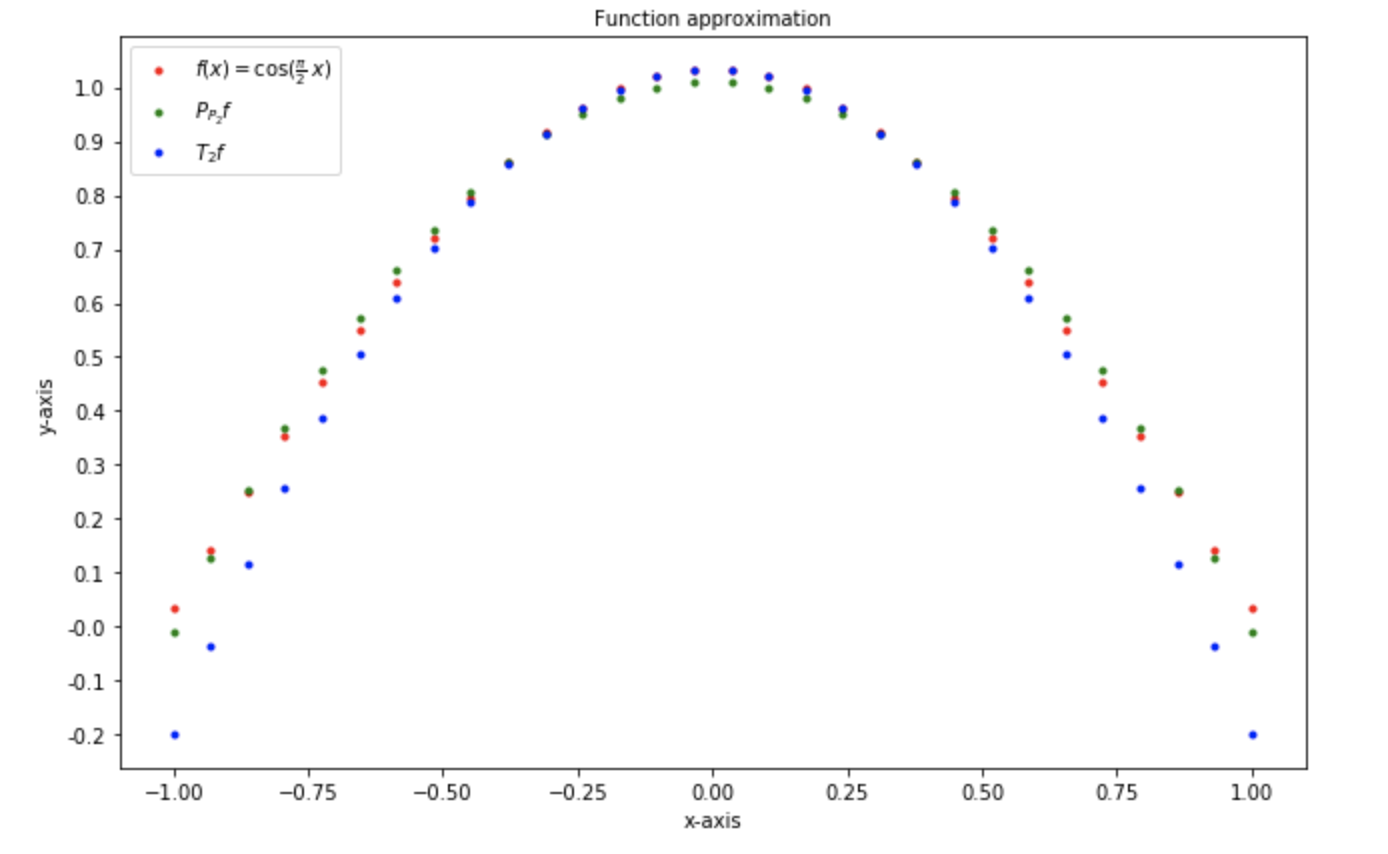
\includegraphics[width=1\linewidth]{figures/problem_3_1.png} 
	\end{center}
	
	\item The plot from the previous part shows that 
    $\ml{P}_{P_2}f$ is a better approximation than $T_2f$
    over most of $[-1,1]$.  Explain why this is the case.
    
    $\mathcal{P}_{P2} f$is the orthogonal projection of $f(x)$ over the subspace of polynomials of degree 2: $\{ w_1, w_2, w_3 \}$, like the Taylor expansion $\mathcal{T}_2 f$. The difference is that the Taylor polynomial is a polynomial expansion of $f$ at 0. So in a neighborhood of $0$, there is almost no differences between $f$ and $\mathcal{T}_2 f$, but as we move away the approximation given by $\mathcal{T}_2 f$ is worst than  $\mathcal{P}_{P2} f$. 
\ee	

\item Scalar linear approximation
\be
	\item First we write $\E[(a x + b - y)^2] = \E[((a x -y) - (-b))^2]$, we know that the best mean-squared error mimimizer of a random variable is its mean so $-b=\E[ax-y] = a \E[x] - \E[y]= a \mu_x - \mu_y$.
	Substituting b in the expression we want to minimize gives us:
	\begin{align*}
		\E[(a x + b - y)^2] 	&= \E[ ( a x - y -  ( a \mu_x - \mu_y) )^2 ] \\
						&= \E[ \{ a (\mu_x - x)  - (y-\mu_y)  \}^2 ] \\
						&= a^2 \E[(x - \mu_x)^2]  + \E[ (y-\mu_y)^2]  -2 a \E[(x - \mu_x) (y-\mu_y)] \\
						&= a^2 \sigma_x^2 + \sigma_y^2 -2\, a\, \Cov(x,y)
	\end{align*}
	Let $f(a) =  a^2 \sigma_x^2 + \sigma_y^2 -2\, a\, \Cov(x,y)$, then $f'(a) = 2 (\sigma_x^2 a - \Cov(x,y))$ and $f''(a) = 2 \sigma_x^2 $.
	The function is strictly convex, and its second derivative is positive, thus its minimizer is $a = \frac{ \Cov(x,y)} {\sigma_x^2} = \rho_{x,y}\, \frac{\sigma_y}{\sigma_x}$.
	
	\item Applying the result from the previous question, the best linear estimate of y given x is $y = \rho_{x,y}\, \frac{\sigma_y}{\sigma_x} (x - \mu_x)  + \mu_y$.
	Notice that $\Var{(x)} = \Var{(y \; z)} = \E{[y^2 \; z^2]} - \E{[y \; z]}^2 = \E{[y^2]}  \E{[z^2]} - \E{[y]}^2  E{[z]}^2 = (\sigma_y^2 + \mu_y^2) \sigma_z^2$ where we have used that a and z are independent and z has zero-mean. And $\E{[x]} = \E[y \; z] = \E[y] \; . \; 0 = 0$. Thus the  best linear estimate of y given x is: $\rho_{x,y} \frac{\sigma_y} {\sigma_z \sqrt{\sigma_y^2 + \mu_y^2}} \; x + \mu_y$.
	 
	 \item If in the expression above of y given x, z is normally distributed with $\sigma_z =1$ then y is perfectly estimated from x.  
 
\ee

\item Gradients
\be
	\item Compute the gradient of $f(x) = b^T x$ where $b \in \mathbf{R}^d$ and $f: \mathbf{R}^d \rightarrow \mathbf{R}$.
	$\frac{\partial f(x)}{x_j} = \sum_i b_i \frac{\partial x_i} {\partial x_j} = b_i$, thus $\nabla f(x) = b$.
	\item Compute the gradient of $f(x) = x^T A x$ where $A \in  \mathbf{R}^{d \times s}$ and $f: \mathbf{R}^d \rightarrow \mathbf{R}$.
	$f(x)	=  x^T A x = \sum_{i=1}^d \sum_{j=1}^d a_{ij} x_i x_j$, then
	\begin{align*}
		\frac{\partial f} {\partial x_k}	&=	\sum_{i=1}^d \sum_{j=1}^d a_{ij} \frac {\partial x_i x_j} {x_k}\\
								&=	\sum_{i=1}^d \sum_{j=1}^d a_{ij} (x_j \delta_{ik} + x_i \delta_{jk}) \\
								&=	\sum_{i=1}^d \sum_{j=1}^d a_{ij} x_j \delta_{ik}  + \sum_{i=1}^d \sum_{j=1}^d a_{ij} x_i \delta_{jk} \\
								&=	\sum_{j=1}^d  a_{kj} x_j +  \sum_{i=1}^d a_{ik}  x_i \\
								&=	(A x)_k + (A x)_k^T
	\end{align*}
	thus $\nabla f(x) = (A + A^T) x$.
\ee

\end{enumerate}

\end{document}
